\begin{figure}[bt!]
    \begin{center}
      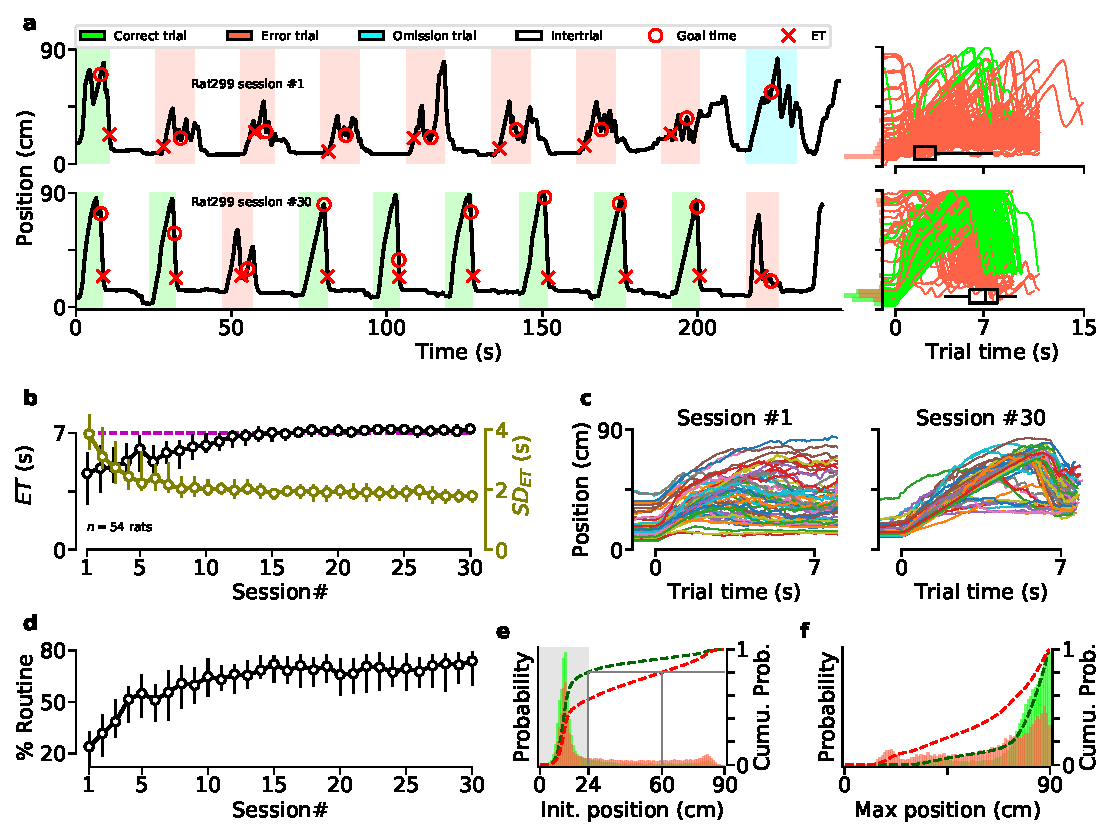
\includegraphics[width=\textwidth]{ch-time/figures/CtrlTrd.pdf}
      \caption[Control Condition]
      {\textbf{Animals developed a unique stereotyped motor sequence.}
      \textbf{a)}
      \textit{Left}: trajectory of a representative animal in 9 consecutive trials of the 1st (\textit{top}) and 30th (\textit{bottom}) sessions.
      On the y-axis, 0~and 90~indicate the treadmills front and rear wall, respectively.
      \textit{Right}: trajectories for all trials of the 1st (\textit{top}) and 30th (\textit{bottom}) session (same animal as in left panels).
      Distributions of initial positions for correct (green) and error (red) trials are shown on the y-axis.
      Black horizontal boxplots depict entrance time range (center line, median; box, 25th and 75th percentiles; whiskers, 5th and 95th percentiles).
      \textbf{b)}
      Median entrance time ($ET$) for the first 30 sessions.
      Circles indicate group median and error bars, the median range (25th and 75th percentiles) across animals for $ET$ and on the right y-axis,$SD$ of $ET$~($SD_{ET}$) values.
      The magenta line shows the goal time (7~s).
      \textbf{c)}
      Median trajectory for the 1st (\textit{left}) and 30th (\textit{right}) training session.
      Each line represents a single animal($n=54$).
      \textbf{d)}
      Percentage of trials in which animals performed the stereotyped routine.
      \textbf{e)}
      Probability distribution function~(PDF) of the position of the animals at the beginning of each correct (green) and error (red) trial, from sessions \#20 to \#30.
      Dashed lines represent cumulative distribution functions (right y-axis).
      The gray area indicates that in trained animals,~80\% of correct trials began with the animal located near the front of the treadmill.
      \textbf{f)}
      PDF of the maximum position along the treadmill.
      Only trials in which animals were initially located in the front of the treadmill (gray area in panel~e) were included.
    }
    \label{fig:time:CtrlTrd}
    \end{center}
  \end{figure}